%!TEX root = ../main/main.tex
\newpage

\section{Deployment View} % (fold)
\label{sec:deployment_view}

In this section we analyze the \emph{Deployment View}, meaning that a presentation of the deployment point of view is provided.

In order to have a successful deployment an in depth analysis of the main components that will have to be deployed is required.
For this reason here is a graph showing the deployment view:
\newpage
\begin{figure}[h!t]
\caption{Deployment Diagram}
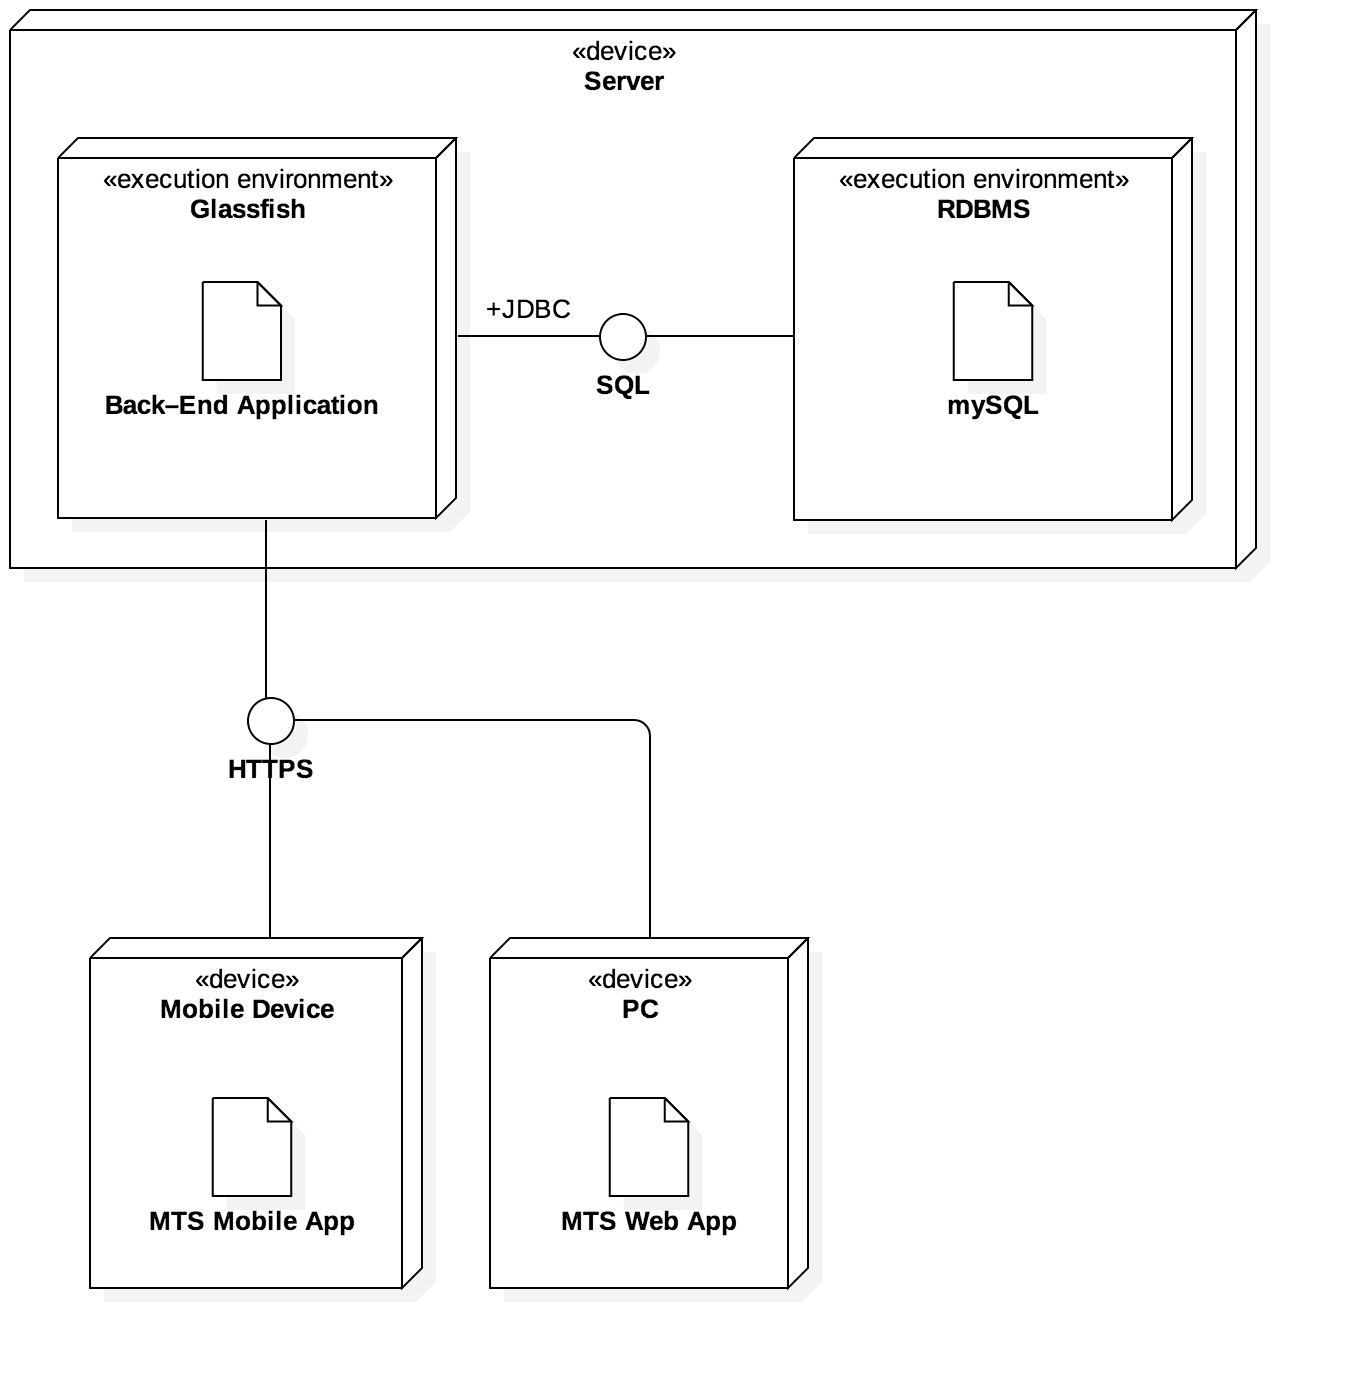
\includegraphics[width=\textwidth]{diagram/png/DeploymentDiagram}
\centering
\end{figure}
\newpage

A main server is deployed, in which the \emph{DBMS} is run. Here also the \emph{Back-End Application} is run via the Glassfish server.

Both mobile applications, the \emph{User} one and the \emph{Taxi Driver} one, interface with the \emph{\nameref{par:back_end_application}} through \emph{HTTP} protocol.

Also the PC application, namely the \emph{Web Application}, connects to \emph{\nameref{par:back_end_application}}.
% section deployment_view (end)